\chapter{Analysis}
\label{chap:analysis}

In diesem Abschnitt wird eine grobe Übersicht über die Software erstellt. Fragen wie, was sind die Anforderungen an die Software, was sind die Anforderungen der Akteure etc. werden hier beantwortet. Ebenfalls wird eine grobe Übersicht über die Programmstruktur erstellt.

\section{Domainmodel}
\label{sec:domain_model}
In diesem Abschnitt wird das Domain Model ("{}Fachmodell"{}) des Mindmap Programmes beschrieben. Es stellt die 
wichtigsten Fachklassen und Assoziationen dar und zeigt die jeweiligen Multiplizitäten.

\begin{figure}[H]
	\centering
		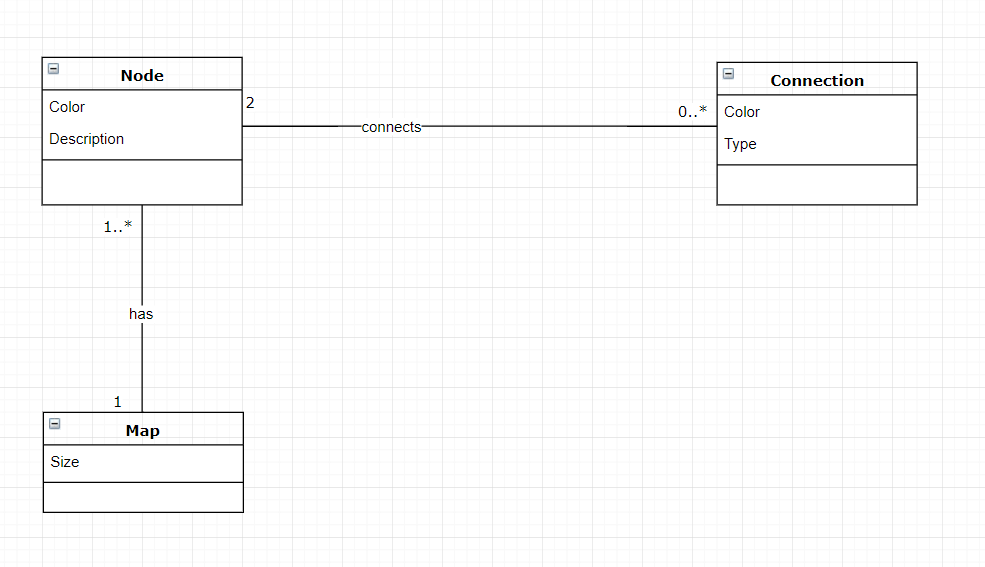
\includegraphics[width=\textwidth]{images/DomainModel.png}
	\caption{Domainmodel}
	\label{fig:domain_model}
\end{figure}

Wie oben in der Grafik zu sehen ist, haben wir uns dafür entschieden, dass eine Map mindestens einen Knoten haben muss um eine Map zu sein. Im Moment denken wir dass die Connection und die Map keine direkte Verbindung benötigen. Dies könnte sich aber beim Implementieren vielleicht noch ändern. Ebenfalls haben wird definiert, dass eine Verbindung immer zwischen 2 Knoten besteht.

\subsection{Assoziationen}
\label{subsec:assoziationen}
\begin{itemize}
\item Zwei Knoten haben keine oder mehrere Verbindungen. Eine Verbindung besteht aus 2 Knoten.
\item Eine Map hat einen oder mehrere Knoten. Ein Knoten gehört zu einer Map.
\end{itemize}

\section{Use Cases}
\label{sec:use_cases}
Use-Cases beschreiben die Requirements der einzelnen Akteure und zeigen die Abläufe des Programmes auf. Dabei wird aber nicht auf die explizite Funktion der einzelnen Teile eingegangen.

\subsection{Use Case Diagramm}
\label{subsec:use_case_diagramm}

\begin{figure}[H]
	\centering
		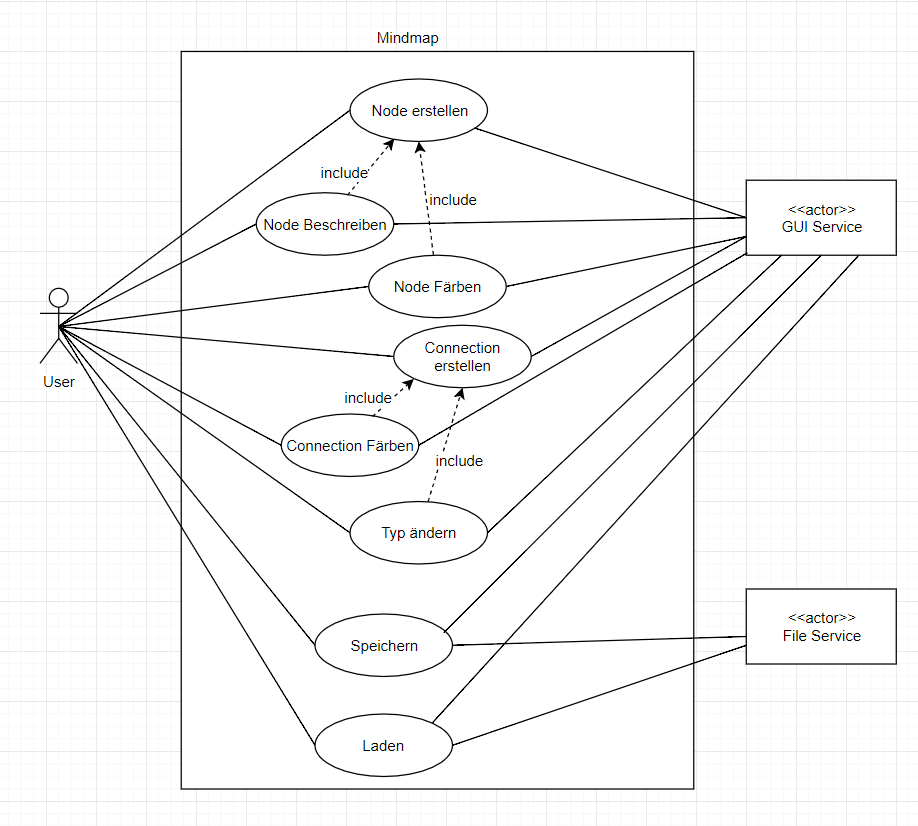
\includegraphics[scale=0.7]{images/UseCaseDiagram.PNG}
	\caption{Use Case Diagramm}
	\label{fig:use_case_diagramm}
\end{figure}

\subsection{Use Cases}
\label{subsec:use_cases}

\subsubsection{Use Case 1: Knoten erstellen}
\begin{itemize}
\item \textbf{Titel:} Als Benutzer möchte ich einen Knoten erstellen können.
\item \textbf{Voraussetzung:} Das Programm ist gestartet.
\item \textbf{Erfolgsszenario:}
	\begin{enumerate}
	\item Der Benutzer gibt den Befehl einen neuen Knoten zu erstellen.
	\item Das Programm fügt den neuen Knoten dem Mindmap hinzu.
	\end{enumerate}
\item \textbf{Nachbedingung:} Ein neuer Knoten wurde dem Mindmap hinzugefügt.
\item \textbf{Alternative Szenarien:}
	\begin{enumerate}
	\item [1.a 1] Der Benutzer schreibt eine Beschreibung für den Knoten.
	\item []
	\item [1.b 1] Der Benutzer ändert die Farbe des Knoten.
	\end{enumerate}
\end{itemize}

\subsubsection{Use Case 2: Knoten verbinden}
\begin{itemize}
\item \textbf{Titel:} Als Benutzer möchte ich zwei Knoten miteinander verbinden können.
\item \textbf{Voraussetzung:} Ein Mindmap mit mindestens zwei Knoten wurde erstellt oder geladen.
\item \textbf{Erfolgsszenario:}
	\begin{enumerate}
	\item Der Benutzer wählt zwei Knoten aus.
	\item Das Programm verbindet die ausgewählten Knoten.
	\end{enumerate}
\item \textbf{Nachbedingung:} Zwischen den ausgewählten Knoten besteht eine Verbindung.
\item \textbf{Alternative Szenarien:}
	\begin{enumerate}
	\item [1.a 1] Der Benutzer ändert die Art der Verbindung.
	\end{enumerate}
\end{itemize}

\subsubsection{Use Case 3: Mindmap speichern}
\begin{itemize}
\item \textbf{Titel:} Als Benutzer möchte ich ein Mindmap speichern können.
\item \textbf{Voraussetzung:} Ein Mindmap wurde erstellt.
\item \textbf{Erfolgsszenario:}
	\begin{enumerate}
	\item Der Benutzer wählt einen Speicherort.
	\item Das Programm übergibt dem Filesystem eine Datei.
	\end{enumerate}
\item \textbf{Nachbedingung:} Eine Datei mit den Informationen des Mindmaps wurde am gewählten Ort im Filesystem gespeichert.
\item \textbf{Alternative Szenarien:}
	\begin{enumerate}
	\item [2.a 1] Das Filesystem verweigert das Speichern wegen zu wenig Speicherplatz.
	\item [2.a 2] Das Programm informiert den Benutzer, dass nicht genug Speicherplatz vorhanden ist.
	\item []
	\item [2.b 1] Das Filesystem verweigert den Zugriff auf den Speicherort.
	\item [2.b 2] Das Programm informiert den Benutzer, dass der Zugriff verweigert wurde.
	\end{enumerate}
\end{itemize}

\subsubsection{Use Case 4: Mindmap laden}
\begin{itemize}
\item \textbf{Titel:} Als Benutzer möchte ich ein gespeichertes Mindmap laden können.
\item \textbf{Voraussetzung:} Eine Datei mit den Informationen eines Mindmap existiert im Filesystem.
\item \textbf{Erfolgsszenario:}
	\begin{enumerate}
	\item Der Benutzer wählt eine Datei aus.
	\item Das Programm lädt die Datei.
	\item Das Programm zeigt das geladene Mindmap an.
	\end{enumerate}
\item \textbf{Nachbedingung:} Das Programm zeigt ein Mindmap mit den Informationen aus der geladenen Datei.
\item \textbf{Alternative Szenarien:}
	\begin{enumerate}
	\item [2.a 1] Das Filesystem verweigert den Zugriff auf die Datei.
	\item [2.a 2] Das Programm informiert den Benutzer, dass der Zugriff verweigert wurde.
	\item []
	\item [2.b 1] Das Programm lädt eine beschädigte Datei.
	\item [2.b 2] Das Programm informiert den Benutzer, dass die Datei beschädigt ist und nicht geladen werden kann.
	\end{enumerate}
\end{itemize}

\subsubsection{Use Case 5: Knoten verändern}
\begin{itemize}
\item \textbf{Titel:} Als Benutzer möchte ich einen erstellten Knoten verändern können.
\item \textbf{Voraussetzung:} Ein Mindmap mit mindestens einem Knoten wurde erstellt oder geladen.
\item \textbf{Erfolgsszenario:}
	\begin{enumerate}
	\item Der Benutzer wählt einen existierenden Knoten.
	\item Der Benutzer schreibt eine (neue) Beschreibung für den Knoten.
	\end{enumerate}
\item \textbf{Nachbedingung:} Der gewählte Knoten wurde verändert.
\item \textbf{Alternative Szenarien:}
	\begin{enumerate}
	\item [2.a 1] Der Benutzer wählt eine (neue) Farbe für den Knoten.
	\end{enumerate}
\end{itemize}

\subsubsection{Use Case 6: Verbindung verändern}
\begin{itemize}
\item \textbf{Titel:} Als Benutzer möchte ich verschiedene Verbindungstypen definieren können.
\item \textbf{Voraussetzung:} Ein Mindmap mit mindestens zwei Knoten wurde erstellt oder geladen.
\item \textbf{Erfolgsszenario:}
	\begin{enumerate}
	\item Der Benutzer wählt eine Verbindung aus.
	\item Der Benutzer ändert die Art/die Darstellung der Verbindung.
	\end{enumerate}
\item \textbf{Nachbedingung:} Die gewählte Verbindung wurde verändert.
\end{itemize}

\subsubsection{Use Case 7: Mindmap drucken}
\begin{itemize}
\item \textbf{Titel:} Als Benutzer möchte ich ein Mindmap drucken können.
\item \textbf{Voraussetzung:} Ein Mindmap wurde erstellt oder geladen.
\item \textbf{Erfolgsszenario:}
	\begin{enumerate}
	\item Der Benutzer gibt den Befehl das Mindmap zu drucken.
	\item Das Programm sendet eine Datei an den Drucker.
	\end{enumerate}
\item \textbf{Nachbedingung:} Das Mindmap wurde ausgedruckt.
\item \textbf{Alternative Szenarien:}
	\begin{enumerate}
	\item [2.a 1] Das Programm informiert den Benutzer, dass kein Drucker angeschlossen ist.
	\item []
	\item [2.b 1] Das Programm informiert den Benutzer, dass die gesendete Datei vom Drucker zurückgewiesen wurde.
	\end{enumerate}
\end{itemize}

\subsubsection{Use Case 8: Mindmap exportieren}
\begin{itemize}
\item \textbf{Titel:} Als Benutzer möchte ich ein Mindmap exportieren können.
\item \textbf{Voraussetzung:} Ein Mindmap wurde erstellt oder geladen.
\item \textbf{Erfolgsszenario:}
	\begin{enumerate}
	\item Der Benutzer wählt ein Dateiformat.
	\item Der Benutzer wählt einen Speicherort.
	\item Das Programm übergibt dem Filesystem eine Datei mit dem gewünschten Format.
	\end{enumerate}
\item \textbf{Nachbedingung:}
\item \textbf{Alternative Szenarien:}
	\begin{enumerate}
	\item [2.a 1] Das Filesystem verweigert das Speichern wegen zu wenig Speicherplatz.
	\item [2.a 2] Das Programm informiert den Benutzer, dass nicht genug Speicherplatz vorhanden ist.
	\item []
	\item [2.b 1] Das Filesystem verweigert den Zugriff auf den Speicherort.
	\item [2.b 2] Das Programm informiert den Benutzer, dass der Zugriff verweigert wurde.
	\end{enumerate}
\end{itemize}

\subsubsection{Use Case 9: Darstellung optimieren}
\begin{itemize}
\item \textbf{Titel:} Als Benutzer möchte ich die Darstellung des Mindmaps optimieren können.
\item \textbf{Voraussetzung:} Ein Mindmap wurde erstellt oder geladen.
\item \textbf{Erfolgsszenario:}
	\begin{enumerate}
	\item Der Benutzer gibt den Befehl das Mindmap zu optimieren.
	\item Das Programm optimiert das Mindmap.
	\end{enumerate}
\item \textbf{Nachbedingung:} Ein Mindmap mit möglichst wenig sich überschneidenden Verbindungen.
\end{itemize}

\section{User Stories}
\label{sec:user_stories}
Eine User-Story beschreibt in ein oder zwei Sätzen eine gewünschte Funktion des Programmes.
\begin{enumerate}
\item Als Benutzer möchte ich, dass das Programm selbsterklärend und einfach zu bedienen ist.
\item Als Benutzer möchte ich ein Programm welches schnell startet und sich nicht langsam anfühlt.
\item Als Benutzer möchte ich ein optisch Ansprechendes Design. Als Benutzer finde ich ein Programm
besser wenn sein Design State of the Art ist.
\item Als Benutzer möchte ich, dass das Mindmap auf dem Papier gleich aussieht wie es im Programm ausgesehen hat.
\item Als Benutzer möchte ich nicht einen Experten konsultieren müssen um ein so triviales Programm zu installieren. 
\item Als Benutzer möchte ich mit dem Programm neue Mindmaps erstellen können.
\item Als Benutzer möchte ich neue Knoten hinzufügen können, welcher eine Beschreibung besitzt und wenn gewünscht auch eine spezielle Farbe haben kann. 
\item Als Benutzer möchte ich die verschiedenen Informationen, also Knoten miteinander vernetzen und so gruppieren können. 
\item Als Benutzer möchte ich meine Arbeit speichern können und gespeicherte Projekte auch wieder laden können
\item Als Benutzer möchte ich die Beschreibung eines Knoten auch nach seiner Erstellung bearbeiten können.
\item Als Benutzer möchte ich die Farbe eines Knotens nach seiner Erstellung bearbeiten können.
\item Als Benutzer möchte ich verschiedene Verbindungstypen definieren können, ich möchte Verbindungen zwischen verschiedenen Themen speziell hervorheben können. 
\item Als Benutzer möchte ich mein Mindmap drucken können.
\item Als Benutzer möchte ich mein Mindmap exportieren können, um es zum Beispiel als Bilddatei in einem Worddokument einfügen zu können.
\item Als Benutzer möchte ich ein Mindmap mit möglichst wenigen überschneidenden Verbindungen, das Programm sollte eine Möglichkeit bieten dieses Problem zu lösen.
\end{enumerate}

\section{Systemkontext}
\label{sec:systemkontext}
Der Systemkontext ist eine Beschreibung des Systems, seiner Teile und äusserlichen Einwirkungen auf das System.

Der Benutzer kann mit unserer Software ein Mindmap erstellen. Dies geschieht über eine grafische Benutzeroberfläche. Mit Hilfe eines Algorithmus können die Themen und Verbindungen des Mindmap optimal verteilt werden. Die Benutzeroberfläche und der Algorithmus sind Teil der Software\\
Die Software greift auf das Dateisystem des Computers zu um ein Mindmap zu speichern oder zu laden. Der Druckservice des Computers erlaubt das Drucken des Mindmaps. Diese beiden Teile liegen ausserhalb unserer Software.

\begin{figure}[H]
	\centering
		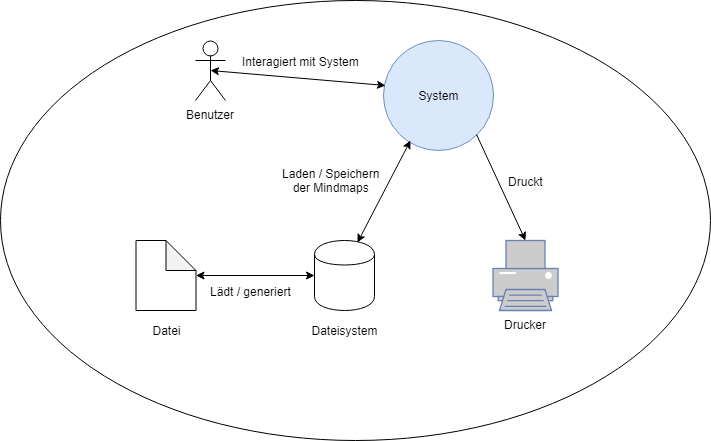
\includegraphics[width=\textwidth]{images/Systemkontext.png}
	\caption{Systemkontext}
	\label{fig:systemkontext}
\end{figure}